\documentclass{svmono}

\usepackage[utf8x]{inputenc}
%\usepackage{cite}
\usepackage{graphicx}
\usepackage{makeidx}
\usepackage{multicol}
\usepackage{footmisc}
\usepackage{ucs}
\usepackage{amsmath}
\usepackage{amsfonts}
\usepackage{amssymb}
\usepackage{textcomp}
\usepackage{epstopdf}
\usepackage{natbib}

\begin{document}
\chapter{MCDM applied to the partioning problem of 3D-stacked integrated circuits}

\section{Introduction}

In order to continuously improve the performance of integrated circuits (IC), technologists have compelled themselves to follow the well-known Moore's Law (see Figure \ref{fig:mooreslaw}). This empirical law predicts a doubling of the transistors' density each 18 months and therefore increasing logic capacity of the circuit per unit area.

\begin{figure}
\begin{center}
\includegraphics[width=0.7\linewidth]{mooreslaw.png}
\end{center}
\vspace{-0.5cm}
\caption{Moore's law \cite{mooreslawpic}}
\label{fig:mooreslaw}
\end{figure}

The improvements of 2D architectures are primarily driven by the reduction of the transistor size. However, with the miniaturization, quantum effects such as quantum tunnelling will significantly affect how a transistor behave. Indeed, even if a transistor is blocking, current can flow through due to quantum tunnelling such that it will be difficult to control its state and thus the basic working principle of a transistor \cite{1240081}. In addition to these physical aspects, economical considerations that will hinder the IC evolution beyond 20nm have to be taken into account \cite{5227192,PFF10}.

In order to overcome these limitations, new technologies have been proposed such as the carbon nanotubes \cite{tans1998room}, the nanowire transistors \cite{doi:10.1021/nl025875l}, the single-electron transistors \cite{citeulike:4194929}, and also the 3D-Stacked Integrated Circuits (3D-SIC) proposed by the academic and industrial communities. The latter has been often cited as the most prominent one as it is based on the current technologies and still uses silicon as basis material; 3D-SICs can also allow shorter interconnection lengths, smaller footprint, larger bandwidth, heterogeneous circuits among their main advantages \cite{659500,1652906,981091,4299568}.

Fast evolution of IC manufacturing technologies makes even the design of 2D-ICs a complex and tedious task with the growing number of design choices at the system level (e.g. number and type of functional units and memories, type and topology of the interconnection system, etc.) and physical level (respecting area/timing/power constraints). Using 3D-SICs introduces even more degrees of freedom: number of tiers, choices for manufacturing technology (e.g. full 3D integration, silicon interposer, face-to-face, back-to-face, etc.), 3D partitioning and placement strategies etc. These new degrees of freedom will contribute to the combinatorial explosion of already huge design spaces. Moreover, practice and 2D design experience cannot be fully exploited with 3D technology, since 3D-SICs change considerably the way ICs are implemented. Indeed, physical implementation of ICs involves solving several complex problems and hence work only with approximated solutions.

Current design flows can produce workable solutions after manual definition of the physical constraints as there are no preconceived method that can provide good solutions. Also, they are sequential in nature as certain parameters are fixed at certain stages in the flow, which can lead to locally optimal solutions that are far from global optimums so this requires time consuming (hence, costly) iterative processes to adjust these parameters. Since the 3D technology is even more complex than the 2D, it is necessary to improve the current design flows by developing design exploration \cite{PFF10}.

One of the solutions to face this problem is to develop high-level tools which can quickly explore design spaces and give early and reasonably accurate performance estimations based on physical prototyping of the 3D circuits~\cite{PFF10}. In addition, performance estimation/optimization and the selection of the most-suitable solutions usually implies to take several objectives into account (e.g. maximization of the performance, minimization of the cost, minimization of the package size, etc.).

Currently, these high-level design tools can be considered to follow a uni-criterion paradigm. Indeed, they have sequential development steps and each criterion is optimized without considering the impact on other criteria. This can lead to several rollbacks in the design flow since the achievement of the requirements can be time consuming (typical design iterations are measured in weeks). For instance, current tools will only minimize the area of a circuit to reach the timing constraints by solving a 2D place-and-route problem and this will be more complex with 3D-SICs because the system has also to be partitioned.

On the other hand, multi-objective approaches have been developed to optimize all the criteria simultaneously. Designing 3D-SICs inherently implies a huge design space and numerous degrees of freedom and criteria, hence many possible choices when it comes to decide upon the IC to produce. With these reasons, we propose in this work to apply a multi-criteria paradigm for the design of 3D-SICs.

\section{Related works}

\subsection{3D-SIC partioning}
%TODO: DRAGO

\subsection{Multi-criteria decision making tools: using the PROMETHEE methods}

In this subsection we recall the basics of the PROMETHEE and GAIA methods. Of course, a detailed description of these approaches goes beyond the scope of this contribution. Therefore we refer the interested reader to \cite{BraMar2005} for a detailed analysis.

Let $\mathcal{A}=\{a_1,a_2,\ldots,a_n\}$ be a set of $n$ alternatives and $\mathcal{F}=\{f_1,f_2,\ldots,f_m\}$ be a set of $m$ criteria. Without loss of generality, we assume that all criteria have to be maximized. The PROMETHEE methods are based on pairwize comparisons. At first, each pair of alternatives $a_i,a_j \in \mathcal{A}$ is compared on every criterion $f_k$:

$$
d_k(a_i,a_j) = f_k(a_i) - f_k(a_j)
$$

The quantity $d_k(a_i,a_j)$ represents the \textit{advantage} of $a_i$ over $a_j$ for criterion $f_k$. On the one hand, when $d_k(a_i,a_j)$ is small enough, there is no good reason to say that $a_i$ is better than $a_j$ regarding criterion $f_k$. On the other hand, when $d_k(a_i,a_j)$ exceeds a certain limit, the decision maker may express that $a_i$ is strictly preferred to $a_j$ for $f_k$. In order to model these statements, the difference $d_k(a_i,a_j)$ is transformed into a unicriterion preference degree, denoted $ P_k(a_i,a_j)$, by using a non-decreasing function $H_k$;

$$
P_k(a_i,a_j) = H_k(d_k(a_i,a_j)), \; \; \forall \; a_i, a_j \; \in \; \mathcal{A}
$$

The quantity $P_k(a_i,a_j) \in [0, 1]$ and $P_k(a_i,a_j)=0$ when $d_k(a_i,a_j) <0$. There are plenty of functions that can be considered to compute the unicriterion preference degrees. In most software implementing the PROMETHEE method, $6$ main functions are considered \cite{Hayez}. Figure \ref{fig:criterion5} represents the so-called linear preference function. Two thresholds characterize it:
\begin{itemize}
\item $q_k$ plays the role of an \textit{indifference} threshold. When the difference $d_k(a_i,a_j) \leq q_k$, it is considered to be so small that the unicriterion preference is equal to zero;
\item $p_k$ plays the role of a \textit{preference} threshold, When the difference $d_k(a_i,a_j) \geq p_k$, it is considered to be important enough to state that $a_i$ is strongly preferred to $a_j$ for this criterion.
\end{itemize}

\begin{figure}[h!]
\begin{center}
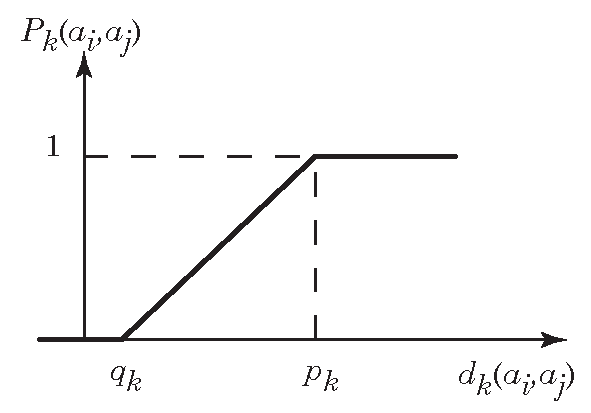
\includegraphics[width=0.7\linewidth]{criterion5.pdf}
\end{center}
\caption{Generalized criterion of type 5}
\label{fig:criterion5}
\end{figure}

Once the unicriterion preference degrees between two actions $a_i$ and $a_j$ have been computed for every criterion, one has to aggregate these marginal contributions to obtain $P(a_i,a_j)$  i.e. a global measure of the preference of $a_i$ over $a_j$:

$$
P(a_i,a_j)= \sum_{k=1}^{m} \omega_k \cdot P_k(a_i,a_j)
$$

where $\omega_k$ represents the relative importance of criterion $f_k$. These weights are assumed to be positive and normalized. Obviously, we have $P(a_i,a_j) \geq 0$ and $P(a_i,a_j) + P(a_j,a_i) \leq 1$.\

The PROMETHEE I and II rankings are based on the exploitation of the matrix $P$. Therefore, three flows are built.; the positive flow $\phi^+$, the negative flow $\phi^-$ and the net flow $\phi$:

$$
\phi^+(a_i)= \frac{1}{n-1} \sum_{a_j \in \mathcal{A}, i \ne j}
P(a_i,a_j)
$$

$$
\phi^-(a_i)= \frac{1}{n-1} \sum_{a_j \in \mathcal{A}, i \ne j}
P(a_j,a_i)
$$

$$
\phi(a_i)=\phi^+(a_i)-\phi^-(a_j)
$$

The PROMETHEE I ranking is obtained as the intersection of the rankings induced by $\phi^+$ and $\phi^-$. The PROMETHEE II ranking is given by the ranking given by $\phi$.

Finally, it is worth noting that:

$$
\phi(a_i) = \frac{1}{n-1} \sum_{k=1}^{m} \sum_{a_j \in \mathcal{A}} {[P_k(a_i,a_j)-P_k(a_j,a_i)]} \cdot \omega_k = \sum_{k=1}^{m} \phi_k(a_i) \cdot \omega_k
$$

where $\phi_k(a_i)$ is called the $k^{th}$ unicriterion net flow assigned to action $a_i$.

The PROMETHEE I and II ranking provide prescriptive tools for decision making. The GAIA \cite{MarBra1988} tool complements them with a descriptive approach. The idea is to represent each alternative by its evaluations in the unicriterion net flow space:

$$
\Phi(a_i)=[\phi_1(a_i),\phi_2(a_i),\ldots,\phi_m(a_i)]
$$

GAIA is the result of a principal component analysis applied on this dataset. Therefore, the decision maker is able to visualize the decision problem on a plane and compare:
\begin{itemize}
\item the relative positions of alternatives (in order to identify groups of similar or distinct alternatives profiles);
\item the relative positions of criteria (in order to identify conflicts or redundancies);
\item the relative positions of alternatives with respect to a given criterion (in order to identify the best and worst alternatives for the different points of views);
\item the relative positions of alternatives with respect to the so-called \textit{decision stick} (in order the identify the best compromise solutions).
\end{itemize}

\section{Case study}
%TODO: DRAGO

\bibliographystyle{plain}
\bibliography{biblio}

\end{document}
